\chapter{Evaluation And Inference}

Training produces a model checkpoint. Evaluation asks how well that checkpoint works. Inference uses the checkpoint to generate text. These are related, but they are not the same job.

A model can have good validation loss and still produce poor samples for some prompts. A sample can look impressive and still hide weak average performance. Good engineering uses both quantitative evaluation and careful qualitative inspection.

\section{Chapter Goals}

By the end of this chapter, you should be able to:

\begin{itemize}
  \item distinguish training, validation, test, and inference workflows;
  \item compute validation cross-entropy and perplexity;
  \item explain how autoregressive generation produces one token at a time;
  \item implement a simple generation loop for TinyGPT;
  \item explain greedy decoding, temperature, top-k, and top-p sampling;
  \item describe why a KV cache speeds up inference;
  \item design reproducible sample reports;
  \item identify common inference failures such as tokenizer mismatch and repetition.
\end{itemize}

\section{Evaluation Versus Inference}

Evaluation and inference use the model differently:

\begin{longtable}{p{0.20\textwidth}p{0.30\textwidth}p{0.34\textwidth}}
\toprule
\term{Mode} & \term{Input} & \term{Output} \\
\midrule
Validation & token windows and targets & average loss/perplexity \\
Test & protected held-out data & final reported metrics \\
Inference & prompt tokens & generated continuation \\
Sampling report & fixed prompt and settings & text plus decoding metadata \\
\bottomrule
\end{longtable}

\begin{center}
\resizebox{0.95\textwidth}{!}{
\begin{tikzpicture}[
  box/.style={draw, rounded corners=2pt, minimum height=0.66cm, text width=2.35cm, align=center},
  arrow/.style={-{Latex[length=2mm]}, thick},
  note/.style={font=\small, align=center}
]
\node[box, fill=blue!5] (ckpt) at (0,0) {checkpoint};
\node[box, fill=yellow!18] (val) at (3.1,1.0) {validation\\loss};
\node[box, fill=green!10] (test) at (3.1,0) {test\\metric};
\node[box, fill=red!8] (infer) at (3.1,-1.0) {inference\\generation};
\node[box, fill=gray!12] (decisions) at (6.4,0) {model\\decision};
\draw[arrow] (ckpt) -- (val);
\draw[arrow] (ckpt) -- (test);
\draw[arrow] (ckpt) -- (infer);
\draw[arrow] (val) -- (decisions);
\draw[arrow] (test) -- (decisions);
\draw[arrow] (infer) -- (decisions);
\node[note] at (3.2,-1.9) {A checkpoint should be judged by numbers and by behavior.};
\end{tikzpicture}}
\end{center}

\section{Validation And Test Sets}

A typical split is:

\begin{itemize}
  \item \term{training set}: used to update parameters;
  \item \term{validation set}: used during development to tune decisions;
  \item \term{test set}: used sparingly for final reporting.
\end{itemize}

If the test set influences many decisions, it becomes a validation set in practice. Honest evaluation requires protecting the final test measurement.

\begin{center}
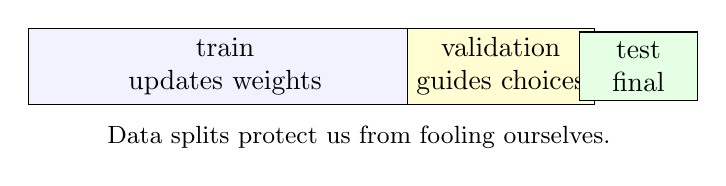
\begin{tikzpicture}[
  part/.style={draw, minimum height=0.7cm, align=center},
  note/.style={font=\small, align=center}
]
\node[part, fill=blue!5, minimum width=5.0cm] at (2.5,0) {train\\updates weights};
\node[part, fill=yellow!18, minimum width=2.0cm] at (6.0,0) {validation\\guides choices};
\node[part, fill=green!10, minimum width=1.5cm] at (7.75,0) {test\\final};
\node[note] at (4.2,-0.9) {Data splits protect us from fooling ourselves.};
\end{tikzpicture}
\end{center}

For tiny educational corpora, validation and test numbers can be noisy. The habit still matters because larger projects depend on it.

\section{Loss As Evaluation}

For language modeling, validation cross entropy is a core metric:

\[
L_{\text{val}}=
-\frac{1}{N}\sum_{n=1}^{N}\log p_{n,y_n}.
\]

Here \(N\) is the number of evaluated next-token predictions. If validation uses \(B\) examples and \(T\) positions per example, then one validation batch contributes \(BT\) predictions.

\begin{center}
\resizebox{0.90\textwidth}{!}{
\begin{tikzpicture}[
  cell/.style={draw, minimum width=0.55cm, minimum height=0.45cm, align=center},
  box/.style={draw, rounded corners=2pt, minimum height=0.62cm, text width=1.9cm, align=center},
  arrow/.style={-{Latex[length=2mm]}, thick},
  note/.style={font=\small, align=center}
]
\node[note] at (1.35,0.65) {validation losses};
\foreach \r in {0,1} {
  \foreach \c/\v in {0/2.1,1/1.8,2/2.4,3/1.9} {
    \node[cell, fill=yellow!18] at (\c*0.65,-\r*0.5) {\scriptsize \v};
  }
}
\node[box, fill=red!8] (mean) at (4.1,-0.25) {average};
\node[box, fill=green!10] (metric) at (6.8,-0.25) {\(L_{\text{val}}\)};
\draw[arrow] (2.75,-0.25) -- (mean);
\draw[arrow] (mean) -- (metric);
\end{tikzpicture}}
\end{center}

Loss is useful because it is objective, cheap, and directly tied to the training objective. But it does not capture every aspect of helpfulness, factuality, safety, style, or instruction following.

\section{Perplexity}

Perplexity is:

\[
\operatorname{PPL}=e^{L_{\text{val}}}.
\]

Intuition: perplexity is roughly the model's average effective number of choices per prediction.

Examples:

\begin{longtable}{p{0.24\textwidth}p{0.24\textwidth}p{0.34\textwidth}}
\toprule
\term{Loss} & \term{Perplexity} & \term{Interpretation} \\
\midrule
\(\log 9\approx2.20\) & 9.0 & uniform guessing over TinyGPT vocabulary \\
1.50 & 4.48 & better than uniform \\
0.70 & 2.01 & quite confident on average \\
0.10 & 1.11 & nearly certain on evaluated tokens \\
\bottomrule
\end{longtable}

For TinyGPT with \(V=9\), random uniform guessing gives:

\[
\operatorname{PPL}=9.
\]

This is a useful sanity check for initial loss.

\section{Evaluation Source Code}

A careful validation function:

\begin{lstlisting}[language=Python]
@torch.no_grad()
def estimate_loss(model, get_batch, eval_iters):
    was_training = model.training
    model.eval()

    losses = {}
    for split in ["train", "val"]:
        split_losses = torch.zeros(eval_iters)
        for k in range(eval_iters):
            x, y = get_batch(split)
            logits, loss = model(x, y)
            split_losses[k] = loss.item()
        losses[split] = split_losses.mean().item()

    if was_training:
        model.train()
    return losses
\end{lstlisting}

Important details:

\begin{itemize}
  \item \texttt{@torch.no\_grad()} avoids storing gradients;
  \item \texttt{model.eval()} disables dropout;
  \item averaging several batches reduces noise;
  \item the previous training/eval state is restored.
\end{itemize}

\section{Inference: Autoregressive Generation}

GPT generation is autoregressive. It produces one token, appends it to the context, then uses the longer context to produce the next token.

\begin{center}
\resizebox{\textwidth}{!}{
\begin{tikzpicture}[
  box/.style={draw, rounded corners=2pt, minimum height=0.66cm, text width=2.05cm, align=center},
  arrow/.style={-{Latex[length=2mm]}, thick},
  note/.style={font=\small, align=center}
]
\node[box, fill=blue!5] (prompt) at (0,0) {prompt\\\texttt{Tiny GPT}};
\node[box, fill=red!8] (model1) at (2.7,0) {model};
\node[box, fill=green!10] (tok1) at (5.4,0) {next token\\\texttt{models}};
\node[box, fill=blue!5] (ctx2) at (8.1,0) {new context\\\texttt{Tiny GPT models}};
\node[box, fill=red!8] (model2) at (10.8,0) {model};
\node[box, fill=green!10] (tok2) at (13.5,0) {next token};
\draw[arrow] (prompt) -- (model1);
\draw[arrow] (model1) -- (tok1);
\draw[arrow] (tok1) -- (ctx2);
\draw[arrow] (ctx2) -- (model2);
\draw[arrow] (model2) -- (tok2);
\node[note] at (6.8,-1.0) {The model is called repeatedly. Each new token becomes part of the next input.};
\end{tikzpicture}}
\end{center}

Generation loop:

\begin{lstlisting}
context = prompt tokens
repeat:
    logits = model(context)
    logits = logits at last position
    probabilities = softmax(logits)
    next_token = decoding_rule(probabilities)
    append next_token to context
\end{lstlisting}

\section{Generation Source Code}

A simple generation function without KV cache:

\begin{lstlisting}[language=Python]
@torch.no_grad()
def generate(model, idx, max_new_tokens, temperature=1.0, top_k=None):
    model.eval()

    for _ in range(max_new_tokens):
        idx_cond = idx[:, -model.config.block_size:]
        logits, _ = model(idx_cond)
        logits = logits[:, -1, :]          # [B, V]
        logits = logits / temperature

        if top_k is not None:
            v, _ = torch.topk(logits, min(top_k, logits.size(-1)))
            logits[logits < v[:, [-1]]] = -float("inf")

        probs = torch.softmax(logits, dim=-1)
        next_id = torch.multinomial(probs, num_samples=1)
        idx = torch.cat((idx, next_id), dim=1)

    return idx
\end{lstlisting}

Shape trace:

\begin{lstlisting}
idx:                 [B, current_T]
idx_cond:            [B, <= block_size]
logits from model:   [B, T, V]
last logits:         [B, V]
probs:               [B, V]
next_id:             [B, 1]
new idx:             [B, current_T + 1]
\end{lstlisting}

\section{Greedy Decoding}

Greedy decoding chooses the most likely token:

\[
x_{t+1}=\arg\max_i p_i.
\]

\begin{center}
\resizebox{0.88\textwidth}{!}{
\begin{tikzpicture}[
  cell/.style={draw, minimum width=0.7cm, minimum height=0.5cm, align=center},
  note/.style={font=\small, align=center},
  arrow/.style={-{Latex[length=2mm]}, thick}
]
\foreach \i/\tok/\p in {0/<pad>/.01,1/<unk>/.02,2/Tiny/.05,3/GPT/.08,4/models/.42,5/learn/.30,6/from/.06,7/tokens/.04,8/. /.02} {
  \node[note, rotate=45] at (\i*0.72,0.8) {\texttt{\tok}};
  \ifnum\i=4
    \node[cell, fill=red!10] at (\i*0.72,0) {\scriptsize \p};
  \else
    \node[cell, fill=blue!5] at (\i*0.72,0) {\scriptsize \p};
  \fi
}
\node[note] at (3.0,-0.85) {Greedy selects the largest probability every time.};
\draw[arrow] (2.88,-0.25) -- (2.88,-0.75);
\end{tikzpicture}}
\end{center}

Greedy decoding is deterministic and useful for debugging, but it can become repetitive because it never explores alternatives.

\section{Temperature}

Temperature rescales logits:

\[
p_i=\operatorname{softmax}\left(\frac{z_i}{\tau}\right).
\]

If \(\tau<1\), the distribution becomes sharper. If \(\tau>1\), the distribution becomes flatter.

\begin{center}
\resizebox{0.92\textwidth}{!}{
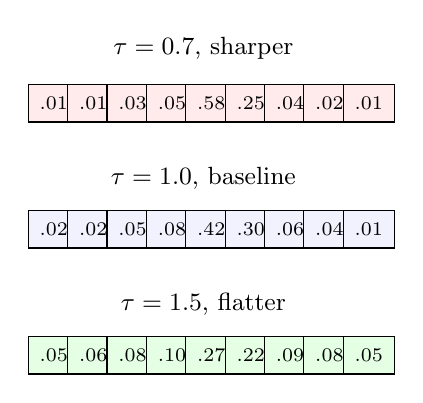
\begin{tikzpicture}[
  cell/.style={draw, minimum width=0.65cm, minimum height=0.48cm, align=center},
  note/.style={font=\small, align=center}
]
\node[note] at (1.9,0.7) {\(\tau=0.7\), sharper};
\foreach \i/\p in {0/.01,1/.01,2/.03,3/.05,4/.58,5/.25,6/.04,7/.02,8/.01} {
  \node[cell, fill=red!8] at (\i*0.5,0) {\scriptsize \p};
}
\node[note] at (1.9,-0.95) {\(\tau=1.0\), baseline};
\foreach \i/\p in {0/.02,1/.02,2/.05,3/.08,4/.42,5/.30,6/.06,7/.04,8/.01} {
  \node[cell, fill=blue!5] at (\i*0.5,-1.6) {\scriptsize \p};
}
\node[note] at (1.9,-2.55) {\(\tau=1.5\), flatter};
\foreach \i/\p in {0/.05,1/.06,2/.08,3/.10,4/.27,5/.22,6/.09,7/.08,8/.05} {
  \node[cell, fill=green!10] at (\i*0.5,-3.2) {\scriptsize \p};
}
\end{tikzpicture}}
\end{center}

Temperature is a generation control, not a training change. It changes how we sample from the model's logits.

\section{Top-k Sampling}

Top-k sampling keeps only the \(k\) most likely tokens before sampling. All other logits are set to \(-\infty\).

\begin{center}
\resizebox{0.92\textwidth}{!}{
\begin{tikzpicture}[
  cell/.style={draw, minimum width=0.65cm, minimum height=0.48cm, align=center},
  note/.style={font=\small, align=center},
  arrow/.style={-{Latex[length=2mm]}, thick}
]
\foreach \i/\p in {0/.02,1/.02,2/.05,3/.08,4/.42,5/.30,6/.06,7/.04,8/.01} {
  \node[cell, fill=blue!5] at (\i*0.58,0) {\scriptsize \p};
}
\node[note] at (2.2,0.65) {original distribution};
\node[draw, rounded corners=2pt, fill=yellow!18, minimum width=1.4cm, minimum height=0.62cm, align=center] (topk) at (6.3,0) {top-k\\\(k=3\)};
\foreach \i/\p/\col in {0/0/gray!18,1/0/gray!18,2/0/gray!18,3/.10/red!8,4/.52/red!8,5/.38/red!8,6/0/gray!18,7/0/gray!18,8/0/gray!18} {
  \node[cell, fill=\col] at (8.0+\i*0.58,0) {\scriptsize \p};
}
\node[note] at (10.2,0.65) {renormalized over top 3};
\draw[arrow] (5.2,0) -- (topk);
\draw[arrow] (topk) -- (7.4,0);
\end{tikzpicture}}
\end{center}

Top-k prevents extremely unlikely tokens from being sampled, while keeping some randomness among plausible tokens.

\section{Top-p Or Nucleus Sampling}

Top-p sampling keeps the smallest set of tokens whose cumulative probability reaches a threshold \(p\). For \(p=0.9\), it keeps enough likely tokens to cover at least 90 percent probability mass.

\begin{center}
\resizebox{0.92\textwidth}{!}{
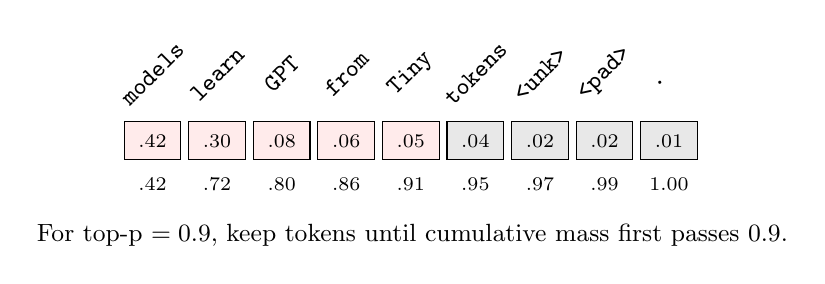
\begin{tikzpicture}[
  cell/.style={draw, minimum width=0.72cm, minimum height=0.48cm, align=center},
  note/.style={font=\small, align=center}
]
\foreach \i/\tok/\p/\cum/\col in {0/models/.42/.42/red!8,1/learn/.30/.72/red!8,2/GPT/.08/.80/red!8,3/from/.06/.86/red!8,4/Tiny/.05/.91/red!8,5/tokens/.04/.95/gray!18,6/<unk>/.02/.97/gray!18,7/<pad>/.02/.99/gray!18,8/. /.01/1.00/gray!18} {
  \node[cell, fill=\col] at (\i*0.82,0) {\scriptsize \p};
  \node[note, rotate=45] at (\i*0.82,0.85) {\texttt{\tok}};
  \node[note] at (\i*0.82,-0.55) {\scriptsize \cum};
}
\node[note] at (3.3,-1.2) {For top-p \(=0.9\), keep tokens until cumulative mass first passes 0.9.};
\end{tikzpicture}}
\end{center}

Top-p adapts the number of allowed tokens depending on confidence. If the model is very confident, it keeps few tokens. If the model is uncertain, it keeps more.

\section{Comparing Decoding Controls}

\begin{longtable}{p{0.20\textwidth}p{0.28\textwidth}p{0.36\textwidth}}
\toprule
\term{Method} & \term{Strength} & \term{Risk} \\
\midrule
Greedy & deterministic, simple & repetitive, dull, local traps \\
Low temperature & focused, stable & less variety \\
High temperature & more variety & incoherence, unlikely tokens \\
Top-k & blocks tail tokens & fixed \(k\) may be too strict or loose \\
Top-p & adapts to confidence & needs threshold tuning \\
\bottomrule
\end{longtable}

There is no universally best decoding setting. Evaluation should report the settings used.

\section{Context Window And Cropping}

GPT has a maximum context length, called \texttt{block\_size}. During generation, the full generated sequence may become longer than this. The simple solution is to crop to the most recent tokens:

\[
\texttt{idx\_cond} = \texttt{idx}[:, -T_{\max}:].
\]

\begin{center}
\resizebox{0.9\textwidth}{!}{
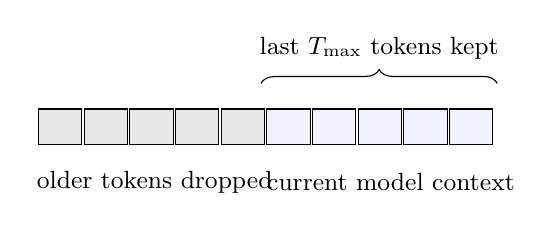
\begin{tikzpicture}[
  cell/.style={draw, minimum width=0.55cm, minimum height=0.45cm, align=center},
  note/.style={font=\small, align=center}
]
\foreach \i in {0,1,2,3,4,5,6,7,8,9} {
  \ifnum\i<5
    \node[cell, fill=gray!18] at (\i*0.58,0) {};
  \else
    \node[cell, fill=blue!5] at (\i*0.58,0) {};
  \fi
}
\draw[decorate, decoration={brace, amplitude=5pt}] (2.55,0.55) -- (5.55,0.55);
\node[note] at (4.05,1.0) {last \(T_{\max}\) tokens kept};
\node[note] at (1.2,-0.7) {older tokens dropped};
\node[note] at (4.2,-0.7) {current model context};
\end{tikzpicture}}
\end{center}

This means a basic GPT cannot directly use information beyond its context window unless a larger architecture or retrieval system is added.

\section{KV Cache}

During generation, recomputing attention over the entire context at every step is wasteful. A KV cache stores previously computed keys and values.

Without cache:

\begin{lstlisting}
step 1: compute attention for 1 token
step 2: recompute attention for 2 tokens
step 3: recompute attention for 3 tokens
...
\end{lstlisting}

With cache:

\begin{lstlisting}
step 1: compute K,V for token 1
step 2: compute K,V for new token; reuse old K,V
step 3: compute K,V for new token; reuse old K,V
...
\end{lstlisting}

\begin{center}
\resizebox{0.95\textwidth}{!}{
\begin{tikzpicture}[
  box/.style={draw, rounded corners=2pt, minimum height=0.62cm, text width=2.2cm, align=center},
  arrow/.style={-{Latex[length=2mm]}, thick}
]
\node[box, fill=blue!5] (old) at (0,0) {cached keys\\and values};
\node[box, fill=yellow!18] (new) at (3,0) {new token\\Q,K,V};
\node[box, fill=red!8] (attn) at (6,0) {attention over\\cache + new};
\node[box, fill=green!10] (out) at (9,0) {next-token\\logits};
\draw[arrow] (old) -- (attn);
\draw[arrow] (new) -- (attn);
\draw[arrow] (attn) -- (out);
\end{tikzpicture}}
\end{center}

For teaching, implement generation without a cache first. For performance, add a cache later.

\section{Inference Across PyTorch, Candle, And llm.c}

Training asks, ``Can the model learn?'' Inference asks, ``Can the learned model become a
reliable product behavior?'' The backend differences matter here too, but the algorithm is
again shared:

\[
\text{prompt text}
\rightarrow \text{token IDs}
\rightarrow \text{prefill}
\rightarrow \text{last-position logits}
\rightarrow \text{sampling}
\rightarrow \text{new token}
\rightarrow \text{repeat}.
\]

During inference, the target \(Y\) disappears. We do not know the next token in advance.
Instead, the model produces a probability distribution
\[
p(x_{t+1}=v \mid x_{\le t}) =
\operatorname{softmax}(\ell_t)_v,
\]
and the sampler chooses a token from that distribution.

\begin{figure}[htbp]
\centering
\resizebox{\textwidth}{!}{%
\begin{tikzpicture}[
    node distance=1.15cm,
    box/.style={draw, rounded corners, fill=blue!7, minimum width=2.6cm, minimum height=0.75cm, align=center},
    runner/.style={draw, rounded corners, fill=orange!13, minimum width=3.0cm, minimum height=0.85cm, align=center},
    outbox/.style={draw, rounded corners, fill=green!10, minimum width=2.8cm, minimum height=0.75cm, align=center},
    arrow/.style={-{Latex[length=3mm]}, thick}
]
\node[box] (prompt) {Prompt\\text};
\node[box, right=0.7cm of prompt] (ids) {Tokenizer\\token IDs};
\node[runner, below right=0.8cm and 0.7cm of ids] (torch) {PyTorch\\research runner};
\node[runner, right=0.7cm of torch] (candle) {Candle/Rust\\product runner};
\node[runner, right=0.7cm of candle] (llmc) {llm.c/CUDA\\systems runner};
\node[box, above right=0.8cm and 0.7cm of candle] (sampler) {Sampler\\temperature, top-\(k\), top-\(p\)};
\node[outbox, right=0.7cm of sampler] (decode) {Decoder\\text};
\node[outbox, below=1.0cm of sampler] (report) {Sample report\\seed, config, backend};

\draw[arrow] (prompt) -- (ids);
\draw[arrow] (ids) -- (torch);
\draw[arrow] (ids) -- (candle);
\draw[arrow] (ids) -- (llmc);
\draw[arrow] (torch) -- (sampler);
\draw[arrow] (candle) -- (sampler);
\draw[arrow] (llmc) -- (sampler);
\draw[arrow] (sampler) -- (decode);
\draw[arrow] (sampler) -- (report);
\end{tikzpicture}}
\caption{Inference should expose the same prompt, tokenizer, checkpoint, sampler, and report format across all backends.}
\end{figure}

\subsection{PyTorch Inference: Best For Inspection}

PyTorch remains the most comfortable environment for inspecting model behavior. A
researcher can pause after each stage:

\begin{itemize}
  \item print prompt token IDs;
  \item inspect logits before softmax;
  \item compare greedy, top-\(k\), and nucleus sampling;
  \item visualize attention patterns;
  \item run ablations by disabling dropout, changing temperature, or cropping context.
\end{itemize}

A PyTorch inference loop is also a debugging bridge back to training. If validation loss
looks good but samples are poor, PyTorch makes it easy to check whether the tokenizer,
checkpoint, device, dtype, or sampler is responsible.

\subsection{Candle Inference: Rust-Native Product Path}

Candle becomes especially attractive at inference time. Many products do not want every
model-serving component to be a Python process. A Rust-native inference runner can share
infrastructure with web services, local desktop tools, command-line utilities, and
embedded model workflows. Candle's ecosystem emphasis on Rust, CUDA support, and
safetensors makes it a serious candidate for this role \cite{huggingfacecandle}.

The key engineering idea is that the Candle runner should not invent a new model. It
should load the same checkpoint contract, tokenizer identity, and config identity used by
the PyTorch reference. The product path should be stricter, not different:

\begin{itemize}
  \item refuse to load a checkpoint with the wrong vocabulary size;
  \item verify tokenizer and config hashes;
  \item record sampler settings in every response log;
  \item provide deterministic greedy decoding for test cases;
  \item expose a small stable API for applications.
\end{itemize}

This is where a training textbook can help industry: it teaches students that model
quality and system reliability meet at the artifact boundary.

\subsection{llm.c Inference: Cache Layout And Throughput Truth}

llm.c-style inference teaches a different lesson: generation speed is often a memory
layout problem. Once the prompt has been processed, each new token reuses previous keys
and values. The KV cache is no longer an abstract idea; it is a set of buffers with
specific dimensions:

\[
K,V \in \mathbb{R}^{L \times B \times H \times T_{\max} \times D_h}.
\]

For a single generated token, the model needs the newest query and all cached keys and
values. A systems backend must decide how those tensors are stored, how they are indexed,
and how kernels read them efficiently. This is why an llm.c/CUDA path belongs beside
PyTorch and Candle: it teaches what changes when the bottleneck becomes memory traffic,
kernel launch overhead, and cache reuse.

\begin{table}[htbp]
\centering
\small
\renewcommand{\arraystretch}{1.25}
\begin{tabular}{p{0.18\textwidth}p{0.25\textwidth}p{0.25\textwidth}p{0.25\textwidth}}
\toprule
\textbf{Inference concern} & \textbf{PyTorch} & \textbf{Candle/Rust} & \textbf{llm.c/CUDA} \\
\midrule
Model loading &
Flexible research checkpoint loading. &
Typed config and safetensors-oriented loading. &
Custom binary or tightly specified buffers. \\
Tokenizer boundary &
Easy to inspect with Python tooling. &
Should be a stable product API boundary. &
Usually external or preprocessed. \\
Tensor device &
Convenient CPU/GPU moves. &
Explicit device selection in Rust. &
Manual device memory management. \\
KV cache &
Simple to prototype and visualize. &
Useful for production-serving discipline. &
Best for studying layout and bandwidth. \\
Sampler &
Fast to experiment with decoding strategies. &
Should expose deterministic, auditable settings. &
Can be optimized after correctness is fixed. \\
Deployment &
Research service or notebook. &
Rust service, local app, or CLI. &
Specialized performance runner. \\
Debugging lesson &
Behavior and probability inspection. &
Artifact compatibility and API reliability. &
Memory/performance mechanisms. \\
\bottomrule
\end{tabular}
\caption{Inference turns backend differences into product, reliability, and performance lessons.}
\end{table}

\subsection{Backend-Invariant Inference Tests}

Every backend should pass the same inference checks:

\begin{enumerate}
  \item The same prompt text encodes to the same token IDs.
  \item The checkpoint, tokenizer, and config hashes match.
  \item A deterministic greedy next-token test agrees on a tiny checkpoint.
  \item The final-step logits have shape \shape{[B,V]}.
  \item Context cropping behaves identically when the prompt exceeds \(T_{\max}\).
  \item Sampling metadata records backend, seed, temperature, top-\(k\), top-\(p\), and
  maximum new tokens.
  \item Reloading the same checkpoint gives the same greedy output.
\end{enumerate}

These tests turn inference from a demo into an engineering artifact. The community does
not benefit from another sample script that merely prints text; it benefits from a
reproducible generation contract that can be implemented in Python, Rust, and C/CUDA.

\section{Tokenizer And Checkpoint Compatibility}

Inference must use the tokenizer that matches the checkpoint. If token ID \(7\) meant \texttt{tokens} during training but means something else during inference, the model's embedding rows and output logits are misinterpreted.

\begin{center}
\begin{tikzpicture}[
  box/.style={draw, rounded corners=2pt, minimum height=0.62cm, text width=2.35cm, align=center},
  arrow/.style={-{Latex[length=2mm]}, thick}
]
\node[box, fill=blue!5] (ckpt) at (0,0.7) {checkpoint\\tokenizer hash A};
\node[box, fill=blue!5] (tok) at (0,-0.7) {loaded tokenizer\\hash A};
\node[box, fill=green!10] (ok) at (3.5,0) {safe to\\decode};
\draw[arrow] (ckpt) -- (ok);
\draw[arrow] (tok) -- (ok);
\node[box, fill=red!8] (bad) at (7,0) {refuse if\\hash differs};
\draw[arrow] (ok) -- (bad);
\end{tikzpicture}
\end{center}

Inference scripts should report:

\begin{itemize}
  \item checkpoint path;
  \item model config;
  \item tokenizer identity;
  \item prompt;
  \item temperature;
  \item top-k or top-p;
  \item random seed;
  \item maximum generated tokens.
\end{itemize}

\section{Qualitative Evaluation}

Samples should be inspected, but carefully. A good-looking sample can hide poor average behavior, and a bad sample can occur by chance. Use fixed prompts and fixed random seeds for qualitative comparisons.

A sample report should include:

\begin{itemize}
  \item model checkpoint;
  \item prompt;
  \item decoding settings;
  \item generated output;
  \item short human notes;
  \item whether the sample is cherry-picked or part of a fixed prompt suite.
\end{itemize}

\section{Common Inference Failures}

\begin{longtable}{p{0.28\textwidth}p{0.48\textwidth}}
\toprule
\term{Symptom} & \term{Likely causes} \\
\midrule
Output is mostly unknown tokens & tokenizer/checkpoint mismatch, bad decoding \\
Repeats same phrase forever & greedy decoding, weak model, low temperature, training data repetition \\
Output is chaotic & temperature too high, top-k/top-p too loose, undertrained model \\
Stops too early & stop token or punctuation handling issue \\
Validation good, samples bad & decoding issue, prompt mismatch, narrow training data \\
Samples differ unexpectedly & random seed or sampling settings not recorded \\
\bottomrule
\end{longtable}

\section{Engineering Practice}

Inference scripts should:

\begin{itemize}
  \item refuse tokenizer/checkpoint mismatches;
  \item call \texttt{model.eval()};
  \item use \texttt{torch.no\_grad()};
  \item crop context to \texttt{block\_size};
  \item record all decoding settings;
  \item support fixed random seeds;
  \item print or save the prompt and decoded output;
  \item optionally emit token IDs for debugging.
\end{itemize}

\section{Hands-On Lab: Compare Sampling Rules}

Use the same prompt and checkpoint. Generate outputs with:

\begin{lstlisting}
greedy
temperature = 0.7
temperature = 1.0
temperature = 1.3
top_k = 3
top_p = 0.9
\end{lstlisting}

Record:

\begin{itemize}
  \item generated text;
  \item repetition level;
  \item coherence;
  \item surprising or interesting tokens;
  \item whether output changes when the seed changes.
\end{itemize}

Explain why randomness can help and hurt.

\section{Hands-On Lab: Evaluate The GPT21 Reference Checkpoints}

The \texttt{gpt21-wikitext103-ddp} run produced many checkpoints:

\begin{lstlisting}
step-500.pt, step-1000.pt, ..., step-9500.pt, step-9999.pt, latest.pt
\end{lstlisting}

This is an ideal evaluation lab because students can see that ``latest'' is not always
the same as ``best.'' From the listed validation logs, step 8250 had the best shown
validation loss:

\[
L_{\text{valid}} = 3.6265,
\qquad
\operatorname{perplexity}=e^{3.6265}\approx37.6.
\]

The final region is still successful, but noisier:

\[
L_{\text{valid at 9750}}=3.8154,
\qquad
e^{3.8154}\approx45.4.
\]

The evaluation task is to build a checkpoint report:

\begin{longtable}{p{0.18\textwidth}p{0.20\textwidth}p{0.22\textwidth}p{0.28\textwidth}}
\toprule
\term{Checkpoint} & \term{Valid loss} & \term{Perplexity} & \term{Decision} \\
\midrule
\texttt{step-8250.pt} & 3.6265 & about 37.6 & candidate best validation checkpoint \\
\texttt{step-9500.pt} & 3.6563 & about 38.7 & near-best, later training state \\
\texttt{step-9999.pt} & not separately listed & compute before release & final milestone checkpoint \\
\texttt{latest.pt} & not enough alone & compute before release & recovery pointer, not proof of quality \\
\bottomrule
\end{longtable}

For each candidate checkpoint, run the same prompts with deterministic greedy decoding
and with one sampling setting such as temperature \(0.8\), top-\(k=40\). Save:

\begin{itemize}
  \item checkpoint path;
  \item validation loss and perplexity;
  \item prompt;
  \item generated text;
  \item token IDs if debugging;
  \item decoding settings and random seed;
  \item backend name: PyTorch, Candle, or llm.c.
\end{itemize}

\subsection{Backend Comparison Rule}

Before comparing sample quality, compare deterministic behavior. PyTorch, Candle, and
llm.c should agree on simple invariants:

\begin{enumerate}
  \item same prompt text produces the same token IDs;
  \item same checkpoint metadata reports the same \(V,T,L,H,C\);
  \item greedy next-token output agrees on a tiny deterministic checkpoint;
  \item logits have the same shape and comparable numeric range;
  \item the sampler receives the same final-position logits.
\end{enumerate}

Only after these checks pass should students compare speed, memory, or qualitative text.
Otherwise, a backend difference may actually be a tokenizer mismatch, checkpoint mismatch,
or decoding mismatch.

\section{GGUF Export Evaluation}

After a checkpoint is selected, it may be exported to GGUF for local inference. This adds
one more evaluation boundary:

\[
\text{training checkpoint} \rightarrow \text{GGUF export} \rightarrow \text{inference runtime}.
\]

The exported file must be treated as a new artifact. It may use a different tensor
packing, different dtype, or quantized weight representation. Therefore, do not assume the
GGUF file is correct merely because conversion finished.

Evaluate the export with a small report:

\begin{longtable}{p{0.24\textwidth}p{0.56\textwidth}}
\toprule
\term{Check} & \term{Question} \\
\midrule
Metadata & Does GGUF report the expected architecture, context length, layer count, heads, embedding size, and tokenizer fields? \\
Tensor inventory & Are all expected tensors present after conversion? \\
Quantization & Is the file FP16, Q8, Q5, Q4, or another type, and was that intended? \\
Prompt parity & Does greedy decoding match the source checkpoint on a tiny deterministic prompt when quantization is not changing results too much? \\
Quality spot check & Do fixed prompts produce coherent outputs comparable to the source backend? \\
Runtime performance & What are tokens/sec, memory use, startup time, and context limit? \\
\bottomrule
\end{longtable}

If the model is quantized, exact logits may not match the original checkpoint. In that
case, compare behavior rather than bitwise equality: perplexity on a small set if
available, prompt outputs, repetition, and failure modes.

\subsection{Conversion Checklist For Evaluators}

When a trained checkpoint becomes GGUF, the evaluator should preserve the chain of
custody:

\begin{lstlisting}
source_checkpoint: checkpoints/gpt21-wikitext103-ddp/step-8250.pt
canonical_export:  exports/gpt21-hf/
gguf_f16:          exports/gpt21-f16.gguf
gguf_quantized:    exports/gpt21-q4_k_m.gguf
source_hash:       ...
gguf_hash:         ...
conversion_tool:   llama.cpp convert_hf_to_gguf.py
quantization:      Q4_K_M
\end{lstlisting}

Then run the same prompt set through:

\begin{enumerate}
  \item the source backend, such as PyTorch;
  \item the full-precision GGUF runtime;
  \item the quantized GGUF runtime.
\end{enumerate}

This separates three questions:

\begin{itemize}
  \item Did conversion preserve the model?
  \item Did quantization change the model acceptably?
  \item Is the target runtime fast and reliable enough?
\end{itemize}

\section{Hands-On Lab: Compute Perplexity}

Suppose validation losses are:

\[
2.20,\quad 1.50,\quad 0.70.
\]

Compute perplexities:

\[
e^{2.20},\quad e^{1.50},\quad e^{0.70}.
\]

Then explain why the first value is close to uniform guessing for TinyGPT with \(V=9\).

\checkpoint

\begin{enumerate}
  \item Why is validation loss not the same as instruction-following quality?
  \item What is perplexity, and how is it related to cross-entropy loss?
  \item Why does autoregressive generation call the model repeatedly?
  \item Why can greedy decoding repeat itself?
  \item What does temperature do to logits?
  \item How does top-k differ from top-p?
  \item Why must generation crop to \texttt{block\_size}?
  \item Why is a KV cache useful during generation?
  \item Why should inference refuse tokenizer/checkpoint mismatches?
  \item What metadata should be saved with generated samples?
\end{enumerate}

\subsection*{Solutions}

\begin{enumerate}
  \item Validation loss measures next-token prediction on held-out data. Instruction-following quality also depends on alignment data, prompt format, reasoning behavior, safety, and user intent.
  \item Perplexity is \(e^L\), where \(L\) is average cross-entropy loss. It can be interpreted as the model's effective average number of choices.
  \item GPT produces only the next-token distribution for the current context. To generate many tokens, each sampled token must be appended and fed back.
  \item Greedy decoding always picks the local maximum. If the model strongly favors a repeated pattern, greedy decoding never explores alternatives.
  \item Temperature divides logits before softmax. Lower temperature sharpens the distribution; higher temperature flattens it.
  \item Top-k keeps a fixed number of highest-probability tokens. Top-p keeps enough tokens to reach a cumulative probability threshold.
  \item The model was built with a maximum context length. Inputs longer than that exceed the position embeddings or attention mask.
  \item A KV cache reuses previously computed keys and values, avoiding repeated computation over the whole context at every generation step.
  \item Token IDs must mean the same thing they meant during training. A mismatch corrupts both embedding lookup and output decoding.
  \item Save checkpoint path, tokenizer identity, prompt, decoding settings, random seed, max tokens, generated text, and notes.
\end{enumerate}
